Let us finally go into detail about the main algorithm. The implementation of this thesis replicates and extends the algorithm proposed by \textcite{Derrac2015} with some novel contributions to deal with the given dataset. Further, some improvements from the works of \textcite{Ager2018} and \textcite{Alshaikh2020} are incorporated, who also replicated and improved the original algorithm and share Prof. Steven Schokaert as last author. According to our evaluation of the field, these two papers provide some useful improvements in several aspects, as they apply the algorithm to different datasets, suggest more straight-forward ways of evaluating their performance, and help in understanding important concepts. That we are focusing on only those three papers should by no means imply that they are the only ones that were considered and influcenced this implementation\footnote{See \autoref{sec:otherwork}}, however in contrast to the other pertinent literature these two works do not substantially divert from the algorithms core principles.
% see \autoref{sec:otherwork} - \cite{VISR12} and their tag genome, the fact that the algorithm detailed here is basically only one step in \cite{Alshaikh2019}, Gärdenfors himself suggested that one may use self-organizing maps instead of classical AI/NLP algorithms.

It is important to keep in mind that the algorithm is no rigid monolith but modularly consists of several components, such as \textit{dimensionality reduction}. Many of these components do not require specific algorithms, and \mainalgos also experiment with different components. The exact system for these components may be exchanged, and in the following these exchangeable algorithms are also referred to as hyperparameters. Note further that while this thesis mostly replicates the work of \textcite{Derrac2015}, the following will describe the algorithm as implemented here, which differs in some details from the original work. For the sake of overview, very specific implementation details will be left out in the following description, as however reproducibility is an important aim for us, implementation details are available in Appendix~\ref{AppendixB} and linked where relevant. \todoparagraph{Further, there is a table that compares the implementations here and in mainalgos, as well as another table what-configs-are-available where, the config-yamls and a section on what-other-things-could-one-have-done-hereandthere.}

\subsection*{Core Algorithm}

\todoparagraph{The following explanation assumes that we accept some things as given. For now we'll do that, but we will later revisit and critically question many of these assumptions!}

% The core idea of the algorithm is to unsupervisedly find a a set of features which can be modelled as directions for a vector-space representation of the respetive entities.
The main goal of the algorithm is to unsupervisedly use text-corpora associated with the considered from a certain domain\glspl{entity}\footnote{From now on, the term \textit{\glspl{entity}} refers to the sample described by one text from the corpus (description, concatenated reviews, ...). The corpus accordingly defines the domain: educational resources, movies, ...} to embed these into a vector-space where the axes correspond to human concepts/Properties.\footnote{\textit{Concepts} and \textit{Properties} explicitly refer to what is defined in Criterions C and P, see \ref{sec:csdefinition}} This is referred to as \textit{feature-based} representation: A high-dimensional vector that numerically encodes the degree (\textit{protoypicality}) to which the entity corresponds to a number of appropriate dimensions. This is generally referred to as Conceptual Space and can be used as basis for explainable reasoning.

The general idea to achieve that is as follows: First, the entities are embedded as fixed-dimensional vectors. To allow for the types of reasoning mentioned in Section \ref{sec:cs_reasoning}, it is embedded into metric spaces where the concepts of direction and distance are well-defined \gencite{Derrac2015} original algorithm uses MDS (see \ref{sec:mds}) for this matter, which enforces metric distances. \cite{Ager2018,Alshaikh2020} both soften this requirement and also use document embedding techniques such as doc2vec and averaged GloVe \todoparagraph{REFERENCE!} embeddings.

Additionally, words or phrases from the text are extracted as candidates for the names of the semantic dimensions. The underlying assumption is that \q{words describing semantically meaningful features can be identified by learning for each candidate word $w$ a linear classifier which separates the embeddings of entities that have $w$ in their description from the others} \cite[3574]{Alshaikh2020}. The better the performance of that classifier according to a chosen metric, the more evidence there is that $w$ describes a semantically meaningful feature. 
% * from Alshaikh2020: "Their core assumption is that words describing semantically meaningful features can be identified by learning for each candi- date word w a linear classifier which separates the embeddings of entities that have w in their description from the others. The performance of the classifier for w then tells us to what extent w describes a semantically meaningful feature"
In a final step, the candidate-words are clustered according to their similarity to find a fixed set of \emph{semantic directions}. A representative term for the directions is selected as dimension name, and the entities are re-embedded into a new space comprised of these dimensions, where the individual vector-components correspond to the ranking of an entity with respect to these dimensions.

The rest of this section goes into further detail for each of the individual components of the algorithm. \removeMe{An overview of which of the considered literature supports each components is given in \autoref{tab:compared_algos}.} Further, configuration files to enable exactly the respective components of the papers \mainalgos for the codebase of this thesis are listed in \aref{ap:yamls_for_origalgos}.

\todoparagraph{but before that, ager and alshaikh}

\removeMe{
\subsection{Regarding ager and alshaikh}

\todoparagraph{describe shortly what the improvements from [2,3] were}

\todoparagraph{Dass die den Zwischenschritt mit dem ganzen geeometric reasoning auf dem interim space nicht machen und DESWEGEN die requirement mit MDS soften konnen}

In principle Derrac2015, but with some components from Ager2018 and Alshaikh2020 as well as some own stuff. I'll be testing some claims or nonclaims of \mainalgos, bspw nutzen sie immer PPMI ohne je tf-idf zu testen. Also of course different nature of the dataset - their "how does this dimension correspond to the count in the reviews" doesn't make sense (their success-metric for the SVM is tailored to the one property, so I expect that one to be worse). I'll elaborate on different ways to deal with that later.
}

\subsection{Algorithm Steps}
\label{sec:algorithm_steps}

% The core idea of the algorithm is to (unsupervised, data-driven) find a a set of features which can be modelled as directions for a vector-space representation of the respective entities. For that, the steps are:

Let us finally describe the steps how to create an interpretable vector-space from the text corpus in detail. For that, we will explicitly elaborate on the parameter choices that branch up at every one. Note that that absolutely is a combinatorical explosion it is impossible to try out all. Further, this is about how this specific implementation does it, which may differ in some details from \mainalgos.

\label{sec:algorithmsteps}
\begin{enumerate}
	\item[\saveref{sec:algo_preproc}{1.}] \textbf{Preprocess} the corpus with default techniques and create a \textit{Bag-of-ngrams representation} (\ref{sec:techniques:bow}) of the texts.
	\item[\saveref{sec:extract_cands}{2.}] \textbf{Extract Candidate Feature} names from words/\glspl{ngram} of the corpus.
	\item[\saveref{sec:generate_vectorspaces}{3.}] \textbf{Embed all Entities} into a fixed-dimensional vector space with demanded properties that captures the respective semantics.
	\item[\saveref{sec:svm_filter_cands}{4.}] \textbf{Filter Candiate Features} by training a linear classifier for each candidate that seperates the vector representations of the entities that contain the term from those that do not. If a specified metric for this classifier is sufficiently high, assume that the candidate term captures a \textit{salient} feature - its direction is then characterized by the orthogonal of the classifier's separatrix.
	\item[\saveref{sec:algo:cluster}{5.}] \textbf{Cluster/Merge the candidates} and calculate the feature direction for each cluster from its components, and (optionally) find a representative cluster-name.
	\item[\saveref{sec:algo:postprocess}{6.}] (optionally) \textbf{Post-process} the candidate-clusters.
	\item[\saveref{sec:algo:reembed}{7.}] \textbf{Re-embed the entities} into a space of semantic directions by calculating their distance to each of the feature direction separatrices.	
\end{enumerate}

This techniques first embeds the collection of texts into a  vector space, to afterwards extract important features from this space using linear classifiers. The second step is an original idea of \cite{Derrac2015}, however creating vector space embeddings from texts is a very popular technique, used for many tasks in \gls{nlp} \cite{Mikolov:Regularities,Mikolov2013a,Guo,Lowe,Turney2010}. This implementation relies on classical creation of the \gls{vsm}, for which the general creation process was explained in \autoref{sec:vsm_construction}. The steps \textit{Build the Frequency Matrix}, \textit{Transform Raw Frequency Counts} and \textit{Smooth the Frequency Matrix} are squashed into the preprocessing and embedding of entities (steps 1 and 3).

 An explicit and simple implementation compliant with each step could be a simple word tokenization and count to generate a bag-of-words (step 1) where each sufficiently frequent word is used as candidate (step 2). A \gls{dissimmat} of the individual \gls{bow}-vectors is compressed using MDS (step 3). A \gls{svm} calculates the accuracy for each candidate (step 4), and k-means-clustering on the 500 top-scoring terms subsequently creates 100 clusters and averages their directions (step 5). The distance to each of the hyperplanes is calculate (step 6), yielding new space for the entities. The sequence of steps is also given as pseudocode in \autoref{ap:algorithm_pseudo}. 
 
 Again it should be stressed that many different components can be considered for each step and the distinction of steps is not rigid: Instead of creating a dissimilarity-matrix followed by dimensionality reduction, \cite{Ager2018,Alshaikh2020} use neural word or document embeddings.\footnote{see \autoref{sec:embeddings}} Instead of extracing candidates from corpus tokens and training a linear classifier for each of them and use their orthogonal as direction, techniques such as LSA or LDA can be employed to find topic vectors directly. We will come back to these ideas when discussing future research opportunities (\autoref{sec:futurework}) by listing what other ways of fulfilling each respective step could have been considered.

\autoref{fig:dependency_graph} shows an automatically exported dependency-graph, displaying the individual steps of the algorithm as done in the accompaning code, also showing where selected important parameters are first used. As explained in \autoref{sec:architecture}, the modularity of the provided architecture allows individual components to be exchanged as needed and run in parallel.


\begin{figure}[H]
	\begin{center}
	  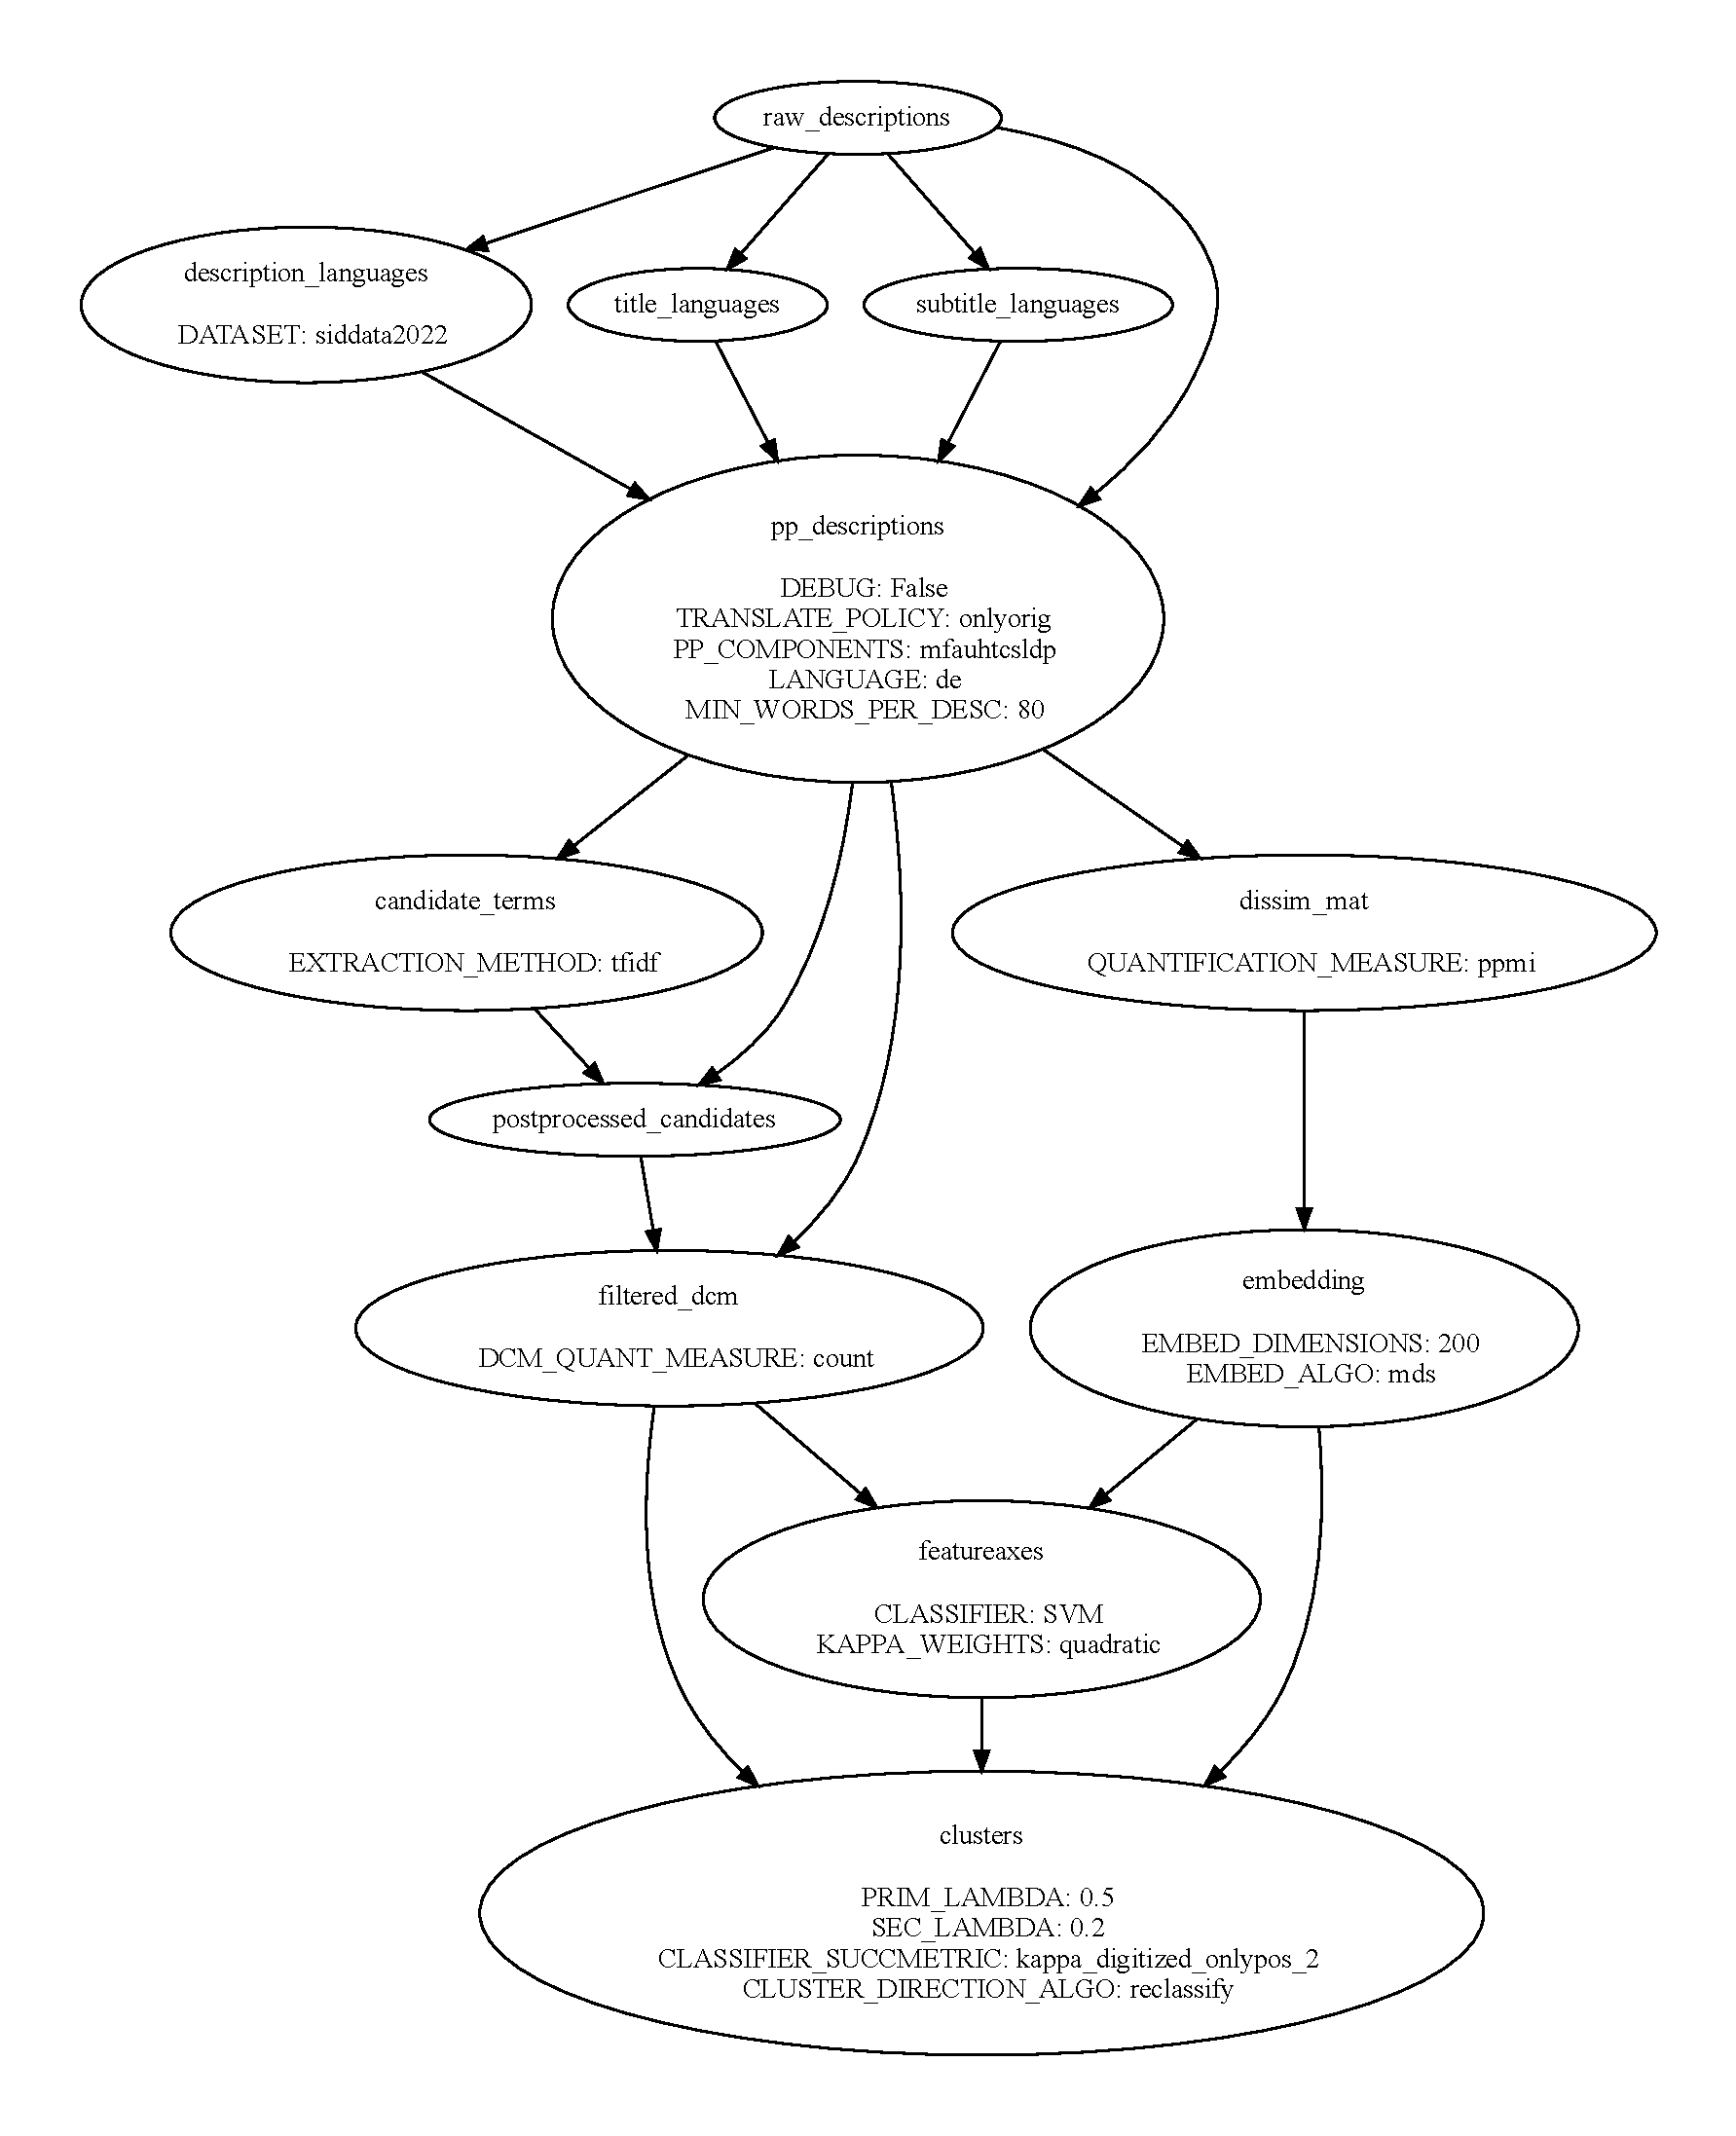
\includegraphics[width=0.9\textwidth]{dependency_graph.pdf}
	  \caption[Dependency-Graph of the Algorithm]{Dependency-Graph of the Algorithm, displaying the individual steps of the algorithm as well as their dependencies and where selected important parameters are first used. \todoparagraph{Generated using command XYZ}}
	  \label{fig:dependency_graph}
	\end{center}
\end{figure}


Before looking at the steps in turn, it should be noted that even the preprocessing does not work on completely raw data, but on curated and processed corpora. This processing is however not considered part of the algorithm, as it is very specific to the respective datasets and manual dataset exploration, tweaking settings such that they are best for each corpus separately. The preprocessing for the Siddata-dataset is described in \autoref{sec:dataset_siddata} and its implementation is done in separate Jupyter Notebooks.\footnote{Such as \url{https://github.com/cstenkamp/derive_conceptualspaces/blob/main/notebooks/create_datasets/Preprocess_Siddata2022.ipynb}}. In the considered literature, the preprocessing is not considered part of the algorithm at all. Their implementations start from already fully processed datasets available as bag-of-words, each separately processed. Details of their individual processing per dataset is listed in \autoref{tab:all_datasets}. By incorporating the preprocessing into the pipeline, this work aims to increase adaptability and reproducibility, and also allows to experiment with different techniques such as translation or lemmatization or how duplicate entities with different associated texts are merged.
% In course-descriptions, I want some parts of the pre-preprocessing be part of the pipeline, like how we merge descriptions of different iterations of the same course that overlap to a high degree (sentwise-merge vs relative-term-frequencies)

\subsubsection{Preprocessing\arrowref{sec:algorithmsteps}}

\label{sec:algo_preproc}

A common prerequisit for NLP algorithms is to pre-process the text corpus. The preprocessing itself consists of multiple independent components chained after each other. Which components are necessary also depends on the processed dataset - as for example the \emph{placetypes}-dataset consists of a collection of \textit{tags} instead of full sentences, tokenizing sentences or removing \glspl{stopword} becomes irrelevant. Other datasets may require additional cleaning or are already available in preprocessed form.

\paragraph{Translation} As the main considered dataset of university-courses is highly multilingual (see \autoref{fig:sid_statistics}), one of the first questions that needs to be addressed is how entities of different langauges are handled. The algorithm consists of classical language processing algorithms such as comparing \gls{bow} representation of the entities, which means that the same text in two different languages may result in maximally different representations (see \autoref{sec:techniques:bow}). Because of this, before any other processing, the languages of each entity is checked, such that those of languages other than the demanded may be either translated, left out or used anyway. For details about the translation, it is referred to Appendix \ref{ap:translating}.\footnote{It should be noted that professional automatic translation is costly and thus not all texts are available in all languages.}

\paragraph{Components} The following components are developed for the preprocessing, every one of which can be individually enabled or disabled:

\begin{itemize}
	\item Prepend title and/or subtitle to the entities' associated text \itemtext{useful for the Siddata-Dataset, as the titles are often quite long and more descriptive than their descriptions}
	\item Remove HTML-Tags from texts 
	\itemtext{useful for the Siddata-dataset, as it includes descriptions for \glspl{mooc} which are crawled from websites and often contain such}
	\item Tokenize sentences 
	\itemtext{such that \glspl{ngram} across sentences are not considered}
	\item Lower-case all words
	\itemtext{reduces the amount of individual words and ensures that words at the beginning of sentences are mapped correctly}
	\item Remove stop-words / frequent phrases
	\item Tokenize words
	\itemtext{means splitting at the word-boundary, resulting in a list of words. Order must be kept in case n-grams are to be extracted.}
	\item \Gls{lemma}tize words
	\item Remove diacritics
	\itemtext{\emph{Diacritics} are glyphs added to basic letters, such as accents or German \emph{Umlaute}. Removing them converts for example the letter \emph{ä} to an \emph{a}}
	\item Remove punctuation 
\end{itemize}

The above can be done either be done with proprietary code for all of these steps,\footnote{Mostly relying on the python package \emph{nltk} \cite{bird2009natural}} or using \codeother{sklearn}\footnote{\url{https://scikit-learn.org/stable/}}s \codeother{CountVectorizer} (which is faster, but less configurable), as \cite{Ager2018} claim to have done.

\paragraph{On Stop-Words}
Removing stop-words from the texts is useful because it makes the resulting frequency more compact and thus less computationally intensive, and stop-words generally have very discriminative power, meaning their occurence among the entities is arbitrary, just making hte emeddings more noisy (cf. \autoref{sec:word_count_techniques}). There are however reasons to not remove them: Two words that are considered stop-words may posess relevant semantic content (such as a \textsc{Fällt aus} in a course title), and also stopwordslists are often incomplete and of low quality \cite{nothman-etal-2018-stop}. For these reasons it is also possible to instead remove \glspl{ngram} that exceeded a certain frequency (\gls{df}).

\paragraph{On Lemmatization}
The languages most prevalent in the considered datasets are considered \textit{agglomerative}, which means word stems are changed by the addition of affixes and suffixes. Consequently, the same word may be present in multiple different forms, which modelled as completely dissimilar vectors in the present \glspl{bow}-approach. Lemmatization is the process of mapping different forms of these words onto the same stem. Considering that the Siddata-dataset consists of far fewer words than the others, this has important implications. For the german descriptions, this implementation relies on the \textit{HanTa} lemmatizer. \todoparagraph{Correct citation for hanta!!} %https://textmining.wp.hs-hannover.de/Preprocessing.html#Lemmatisierung

The result of this step is a bag-of-ngrams representation for each entity (see \autoref{sec:techniques:bow})


\subsubsection{Extract Candidates\arrowref{sec:algorithmsteps}}
\label{sec:extract_cands}
% Section 4.2.1 of Derrac2015

The final result of the algorithm is a metric space in which the individual dimensions (\emph{\glspl{feature}}/\emph{Interpretable direcitons}) correspond to natural-language concepts and attributes. The candidates for these features are verbatim phrases extracted from the text-corpus of the \glspl{entity}, which are subsequently filtered and merged as necessary.

In \gencite{Derrac2015} work, the selection of phrases to be extracted depends on the dataset: For placetypes-dataset, all sufficiently frequent\footnote{\label{fnote:cand_thresholds}The respective thresholds are listed in \autoref{tab:all_datasets} as ``candidate word threshold''.} 1-grams\footnote{Note that in the case of the place-types dataset, a 1-gram corresponds to all merged words of a tag.} were considered. For the other two datasets, they applied a \gls{pos}-tagger that extracted all sufficiently frequent\footnoteref{fnote:cand_thresholds} \textbf{adjectives, nouns, adjective phrases} and \textbf{noun phrases}, assuming that adjectives would correspond to gradual properties (\eg \textit{violent, funny}) and nouns to topics (\eg the \textit{genre}) \cite[Sec. 4.2.1]{Derrac2015}. Also, the authors ensured that the number of extracted candidates for both datasets is roughly equal, getting around 20\,000 candidates for movies and placetypes.

% Their method depended on the dataset - as their placetypes-dataset was just a collection of tags and the number of tags with term-freq >= XYZ (docfreq>2?! hä?) corresponded to their desired number of candidates anyway (around 22k), they just took all of these as candidates. For their movie-reviews-dataset, they considered all nouns, adjectives, nounphrases 	and adjective-phrases as detected by a POS-tagger. Doing something similar in the scope of this thesis led to suboptimal results, which is why alternative methods were developed
For this step, the implementation of this thesis differs from the original algorithm, as both taking all words as candidate and running a \gls{pos}-tagger led to suboptimal results in previous experiments, which indicated that the robustness of the algorithm is increased if less candidates are considered in earlier steps. This will be further argued and elaborated in the discussion. To ensure comparability to these works however, in the case of the placetypes-dataset the original method of taking all words with a term-frequency of at least 50 was used. Similar techniques for the Siddata-dataset were also considered, but in constrast to the placetypes-dataset it is also important to consider various-length n-grams. While \textcite{Derrac2015} claim to have considered \glspl{ngram} for the movies-dataset, the published version of this dataset contains a \glspl{bow}-representation for each entity where the original word-order is lost, making it impossible to recover \glspl{ngram}, making comparisons with their results impossible for that dataset.\footnote{\url{https://www.cs.cf.ac.uk/semanticspaces/}}

% \todoparagraph{thing is I have less words but the algorithm seems to profit from less words as that makes it more robust}
% I would however argue that the difference here doesn't make a relevant difference 

In our implementation the candidate-extraction is split into four subsequently excecuted substeps, because depending on the algorithm used to extract the candidates the runtime of the individual components is comparably long and some settings are only relevant in later substeps. The steps are:
\begin{itemize}
	\item Extracting Candidate Terms
	\item Postprocessing the Candidates
	\item Creating the \gls{doctermmat} for the candidates and applying a \gls{quant}
\end{itemize}

As visualized in \autoref{fig:dependency_graph}, these substeps only depend on the preprocessed descriptions, which means they can be run in parallel to the creation of the embedding.\footnote{\todoparagraph{Another good reason for cluster exceution!}}

% This can be done either based on the frequency (meaning all terms with a minimal term-frequency), based on some notion of *importance* (based on scores like tf-idf or ppmi), or by more complex means of figuring out *important* keywords and keyphrases. An example of the latter would be KeyBERT
Three main techniques are implemented to extract candidates from the text-corpus. Irrespective of the algorithm, only words with a sufficiently high \gls{df} are extracted, which is important to ensure that the classifier that determines its meaningfulness has enough samples in both clases. This means that the minimal freqeuncy can be calculated from the dataset size: In \cite{Derrac2015}, the minimal frequency for the movies-dataset with 15\,000 entities was only 100, meaning that the algorithm even works if only 0.6\% of samples are in the positive class. 

\todoparagraph{We will come back to this later}
\todoparagraph{HAB ICH DF UND TF RICHTIG??}

\begin{description}
	\item[By frequency:] consider all phrases that exceed a specified document-frequency (like \cite{Derrac2015}).
	\item[By a \gls{quant}:] consider all phrases that are prominent by some notion of \textit{importance} , such as the \gls{ppmi} or \gls{tf-idf}-score. Note that the respective scores depend on the combination of document and term, such that candidates may be extracted for some documents. Of course, all their occurences are considered in the creation of the frequncy matrix.
	\item[Using \emph{KeyBERT}\cite{grootendorst2020keybert}:] consider phrases whose BERT-embedding \cite{Devlin2019} is most similar to the text they are in. 
\end{description}

Using KeyBERT results in candidate terms that are most appealing in qualitative inspection, however it is also most computational demanding, techniques and requires substantial amounts of post-processing for the resulting phrases. More details on KeyBERT and how it is incorporated into the algorithm are given in the implementation are given in Appendix~\ref{ap:details_keybert}

Finally, a \gls{doctermmat} is created from the postprocessed candidates, containing the frequency for each candidate-phrase in each entity. The creation of this frequency matrix mirrors the process described in \autoref{sec:vsm_construction}, however only for the extracted words. After filtering this matrix to ensure that only candidates with a minimal \gls{df} or \textit{stf} are considered, a quantification is applied as described in \autoref{sec:word_count_techniques}. Available Quantifications include raw count, binarization\footnote{meaning all counts are either one or zero. According to \cite{Alshaikh2020} this improves performance \todoparagraph{Aber ich hab logische Probleme damit}}, tf-idf or PPMI.

\cite{Derrac2015} \todoparagraph{always only use PPMI without ever testing tf-idf or giving a reason, I'll try both}

\todoparagraph{so the relation of term to document may be expressed by something else than count - so if we later compare the ranking induced by the svm to this maybe something else thatn the count stands there - I'm expecting that for my dataset tf-idf is much more valuable than the count bc no concatenated reviews or tags}


\subsubsection{Generating Vector Space Embeddings\arrowref{sec:algorithmsteps}}
\label{sec:generate_vectorspaces}

\todoparagraph{This is Turney2020s "Building the frequency matrix", BUT SO IS THE STEP ABOVE}

In this step, the individual \glspl{entity} are embedded into a fixed-dimensional vector space, making up a \emph{frequency matrix}. Importantly, while this matrix is a \gls{doctermmat}, it is only an interim result in the algorithm and the calculation of distances and directions will be done on another matrix from a later step - This is where our pipeline starts to diverge from what the pipeline specified in \nameparanref{sec:vsm_construction}. So we created a frequency matrix that encodes the relevance of a candidate-phrase for each entity in the previous step, and in this step we create another one that encodes each document as a vector. Neither of these matrices will be used to finally calculate similarities on, but both are important to get the dimensions necessary for for these similarities.

Embedding words, \glspl{ngram}/phrases or other tokens, as depicted by \cite{Turney2010,Lowe}, generally involves counting the token frequencies, transforming them to get relative frequencies, and performing dimensionality reduction on the resulting matrix.
So far (step 1), we have counted the token frequencies. 
\todoparagraph{yes we are talking about all tokens}
\textcite{Derrac2015} argued that this space must be a Euclidean \todoparagraph{which is invariant to affine transformations}, such that geometric/algebraic solutions correspond to commonsense commonsense reasoning tasks (see \autoref{sec:reasoning}). \todoparagraph{We will later look into this in more detail}. 
Another requirement is that the number of dimensions is can be chosen as hyperparameter to the algorithm to be able to find a compromise between \todoparagraph{powerfulness and compression... nee argh was fur worter suche ich hier... drauf zuruckkommen wenn ich den teil uber vsms fertig hab. ausserdem, reicht das schon als beschreibung dann?}. Because of these two requirements, \todoparagraph{and also because gardenfors said so} they selected \gls{mds} for dimensionality reduction.

As stated in \autoref{sec:mds}, \gls{mds} calculcates a Euclidean \gls{vsm} from a set of pairwise distances. This means that the algorithm first creates a \textit{Dissimilarity Matrix} that encodes the distance between all pairs of entities (represented as Bag-of-ngrams representation), from which subsequently the final embedding is generated.  
\todoparagraph{This technique of bag-of-ngrams-representation then dissimmat and quantication is not the only way to do it, ager and alshaikh both did it differently}

\todoparagraph{Note that we can use another quantification than in the step above! In my algo this sometimes performed best.}
\todoparagraph{do all this again argh}

In their algorithm, the dissimilarity-matrix is created using distance metrics for the bags-of-words of the respective entities. 

\paragraph{Document embeddings}
If the strict requirement for a metric space is dropped however, many different algorithms may instead be used at this point - not only different dimensionality reduction methods for the embedding, but also ones that do not rely on the distance matrix or even the \gls{bow} at all, like document-embedding-techniques such as \gls{doc2vec} \cite{Le2014} (as \eg used by \cite{Alshaikh2020}). This would change only these steps and the rest of the algo not too much.
However when \cite{Alshaikh2020} used doc2vec instead of dissimmat-mds, it performed worse (see tables in results), which is why it is not in this thesis 


\paragraph{Create Dissimilarity Matrix and Quantify}

The default way of doing it is to create a \gls{doctermmat} that counts the occurences for all words\footnote{Not just the candidates in step 2, but words that occur in any description} for all entities.

In their algorithm, the \gls{dissimmat} is created using the \emph{normalized angular distances} of the \glspl{bow} of the respective entities.  

From this quantified Doc-Term-Matrix, a dissimilarity-matrix is generated. This requires a measure for the dissimlarity - in the original paper, this is what they call "normalized angular difference" - according to \cite{Derrac2015}:

\begin{align}
	ang(e_i, e_j) &= \frac{2}{\pi} * \arccos \left( \frac{\vec[m]{v_{e_i}} * \vec[m]{v_{e_j}}} { \lVert \vec[m]{v_{e_i}} \rVert * \lVert \vec[m]{v_{e_j}} \rVert }  \right)  \label{eq:norm_ang_dist} \\
	&= \frac{2}{\pi} * \arccos(1-\cos(\vec[m]{v_{e_i}},\vec[m]{v_{e_j}})) \text{, where $\cos$ is the default cosine-distance} \nonumber
\end{align}

in \cite{Schockaert2011}, they define similarity through a variation of the Jaccard-distance (IoU, Overlap-Area divided by Union-Area)

\paragraph{Embed}

Because this dissimilarity-Matrix is far too high-dimensional and sparse, a dimensionality-reduction is applied - we discussed other raeasons why that is smart before.

Multidimensional scaling but also isomap yadda yadda


\subsubsection{Filter Candidates by Classifier Performance\arrowref{sec:algorithmsteps}}
\label{sec:svm_filter_cands}

\todoparagraph{Also known as: Creating Candidate SVMs and Filter Candidate Feature Direcitons}
\autoref{ap:algo_filter}

This step brings together the entity embeddings and the extracted keyphrases. To quantify how well each semantic directions captures semantic content of the entities, a linear classifier splits those entities where the keyphrase occurs from those where it does not. The best example for such a classifier is a \gls{svm} which does not rely on the kernel trick.\footnote{kerneltrick ist ja "Projecten in nem anderen space, damit das was da linear ist bei uns nonlinear ist" und ich will linear sein)} As visually exemplified in \autoref{fig:3d_hyperplane_ortho}, the result is a hyperplane that divides the positive and negative samples (the plot a toy-example - in practice it is highly unlikely that they are clearly distinct, but the properties hold in other cases as well). Regardless of the dimensionality of the original space, this hyperplane has a one-dimensional orthogonal vector. Each of the entity-embeddings is subsequently orthogonally projected onto this orthogonal. Now the distance of this projection to the plane offset (the coordinate where it crosses the decision surface) is a scalar that encodes the distance to this decision hyperplane. \footnote{Again, if you don't understand this, look at the plot}

The ranking of the entities in terms of this distance is now what is used as their values for the feature directions, in the sense that the further away an entity is from the decision surface on the positive side, the more it has the corresponding feature. The same holds for the negative direction. This may sound initially surprising, but the point is that the original space is created based on similarity measures of the entities. Given that the \textit{Bag-Words-Hypothesis} (\autoref{sec:bow_hypothesis}) holds, they should have similar words. And those that are maximally dissimilar are as far apart from these as the space allows. To stick with the example of movies, the assumption is that movies that are maximally unscary are maximally far from the away from scary ones, in the sense that you can assume that a maximally dissimilar distribution of words from the positive class means a maximally unscary movie. So the more dissimilar to that, the less scary, so the relationship holds in both directions, even if the word scary itself occurs zero times in the descriptions of any movie on the negative class it still holds that the further away the less the concept applies. Distributional Hypothesis and what we wrote for the logic of LSA. The classifier takes the other words into account for the classification as well. The logic of this is especially clear in the case of SVMs: This classifier works by creating the hyplane such that hte margin between the positive and negative class is maximized. 

Ok so the orthogonal to the resulting decision-hyperplane is then used as axis, onto which the entities are mapped - the further away from the plane the mapping of a point onto the orthogonal, the more the entity is said to have the attribute encoded by the phrase responsible for the hyperplane. A score function compares the ranking induced by this to the ranking induced by number of occurences (or quantification-value) of the respective keyphrase of all documents, such that only those terms where the correspondance of these rankings exceeds a certain threshold are considered as candidate directions henceforth.

\q{The higher the Kappa score of a term \textit{t}, the more we consider \vec{v_t} to be a faithful representation of the term \textit{t}} \q[20]{Derrac2015}. Subsequently only those directions are considered where this classifier exceeds a certain threshold. So what's the logic behind that? As we stated before \todoparagraph{When discussing bow-representations and the reasons for quantifications and also LSA and also stop-words}, unimportant words are more or less uniformly, in any case arbitrarily, distributed throughout the corpus. The vector space that we are doing this SVM on is created on the basis of distributional semantics. The entire basis of this is that there are latent obfuscated topics, and correlations of words for these. So if a topic is very prominent in some texts but not in others, that will influence the position in the vector space. In the case of unimportant words, they are arbitrarily distributed and are not signifying a latent topic, no correlation of other words, not important for similarity. Like no reason for dissimilarity. Not indicating a cluster, because all these stopwords occur random and are thus noise. These randomness does not go along with a cluster of positions in any of the dimensions, nose gets removed by dimensionality reduction. So yes, it does make sense that the better a classifier can split between does-the-word-occur and does-it-not, the more the word is an \textit{important topic} in the sense that it explains the dissimilarity in the entities.\footnote{For a better intuition why this makes sense it is referred to \cite{Lowe}}
\todoparagraph{Do I need a plot that shows a non-faithful direction? } % grafische Darstellung von "if the ranking induced by the SVM corresponds to the count/PPMI, we see it as faithful measure", also ein beispiel wo's passt und ein Beispiel wo's nicht passt

\cite{Ager2018}: \q{if this classifier is sufficiently accurate, it must mean that whether word w relates to object o (i.e. whether it is used in the description of o) is important enough to affect the semantic space representation of o. In such a case, it seems rea- sonable to assume that w describes an important feature for the given domain.}



Okay so lets continue.

Concretely, the score used by \cite{Derrac2015} to assess the performance is not the accuracy or some other measure of the bare performance of the classifer, but rather if the ranking by distance to decision hyperplane corresponds to ranking of number of occurences (or the PPMI-score, the authers are imprecise in their wording) of that word.
The reasoning behind that becomes especially clear when considering the root of their datasets - in the case of reviews or tags it is the case that the often a word is mentioned, the more relevant the word is for that entity. And because we are using the PPMI-score, it is even more: The more salient relevant for this entity but not for the others the word is, the higher the score. That is what how we created the semantic space in the first place, by saying important ones are weighted more, those are very prominent for some but not all were important for the dissimilarity that is the basis for our embedding. So this entire thing basically looks back at our embedding and tries ot figure out which words it were that were relevant for the dissimilarity. It dissects the overall dissimilarity we had before into its components.

Okay, enough for the theory, lets talk about the implementation. \cite{Derrac2015} say that they use the Kappa-score, which is a metric that compares rankings. With that, they compare the rankings of the svm with the ranking how-important that word is. They took kappa because that is good at dealing with high imbalances in class sizes, which are definitely given.

Yet another point where \cite{Derrac2015} are really low on information what parameters they used. Sklearn allows different weighting types\footnote{\url{https://scikit-learn.org/stable/modules/generated/sklearn.metrics.cohen_kappa_score.html\#sklearn.metrics.cohen_kappa_score}} 
\todoparagraph{explain what that changes respectively}

Unfortunately, they give hardly any details, and there are many different ways how to implement that. While \cite{Ager2018,Alshaikh2020} explicitly say that they are interested in the PPMI-scores\footnote{Though the uploaded code of \cite{Alshaikh2020} does not compare rankings but raw values}, from \cite{Derrac2015} it is not even clear if they take the count or the PPMI-score. As that is highly relevant, we try many different ways of this scoring and report them in the results. We also compare the overlaps of different kappa-scores to check if the choice is as imporant as we think it is. Which scores we used and how they are written here is listed in the implementation details: \autoref{tab:kappa_measures}.

\textcite{Ager2018} compare the kappa-score to accuracy and NDCG and say accuracy works better than kappa.

So, alogorithm: For every candidate-term, take the quantifications from the doc-term-matrix and binarize it, such that we have two classes. On that we then train a linear classifier such as an SVM. On that we calculate binary classificaiton-quality-metrics, and from the ranking the kappas. resulting SVM has a hyperplane as decision surface. The distance of a point to it's orthogonal projection onto that hyperplane can be seen as proportional to how much this point is considered to be in the respective class of the SVM. One can use these distances to enduce a ranking how prototypicality. compared to other heuristics encoding it, such as the ranking induced by the per-term-frequencies of the terms for all documents, or it's PPMI or tf-idf representations.
\cite{Derrac2015} call this "measure the faithfulness of representation"

\cite{Ager2018}: \q{We say Feature *Directions* and not feature *vectors* because they are supposed to rank, not measure degrees of similarity! it only tells us "this one has the feature to a higher degree"}


In the end we have a shitton of scores, and two threshold, yielding great ones and okay ones.
Ehm, why didn't I just take the ndims*2 best ones instead of hard-thresholding??
Well, I can say it was because:

At this point we already have an estimate of how good the parameter-combination so far was: if not enough great-ones were extracted, we don't need to bother continuing.



\includeMD{pandoc_generated_latex/3_1_algorithm}




\subsubsection{Merging the extracted candidate-directions\arrowref{sec:algorithmsteps}}
\label{sec:algo:cluster}

The previous step yielded many \textit{basic feature directions} that are defined as direction of the orthogonal vector for the hyperplanes splitting each individual candidate \gls{ngram}. The performance-thresholds are set such that many more directions are generated than the demanded dimansionality of the final embedding, such that they must be clustered and merged.

This is done via the following substeps, each of whch will be closer eloaborated:

\begin{itemize}
	\item Cluster good-performing candidates by their similarity
	\item (optional) Remove uninformative features
	\item Recalulate the direction of the cluster
	\item (optional) Find a representative name for the cluster
\end{itemize}

\paragraph{Clustering the candidates}

Clustering refers to an unsupervised algorithm that groups items based on some notion of similarity. In our case the assumption is that semantically similar concepts have \textit{close} vectors, which is given due to the \gls{bow}-hypothesis that states that the underlying structure of our dataset is expressed by the usage of related words ((\autoref{sec:bow_hypothesis}), \ref{sec:lsi}).\footnote{In case of the Siddata-dataset, it may mean that in courses that contain the word \textit{computer} have a high chance of also containing \textit{program}.} As these vectors in principle only encode a direction, their similarity can be calculated by their \gls{cos}.

The clustering should reduce the number of features and also ensure that the resulting directions are different enough. Note that unlike \eg in Principal Component Analysis (PCA), the suggested here techniques do not enforce orthogonality, such that the resulting directions may remain linearly dependent to a certain degree. As in the final embedding only the projection onto those directions is relevant, it must be ensured that enough of the data's original variation is covered by these directions. To ensure that, we follow \gencite{Derrac2015} suggestion to allow for redundancy by extracting twice as many directions than the original \gls{vsm} dimensionality. 

This implementation implements the original clustering-method of \cite{Derrac2015}:

First, we consider the best \textit{basic features} as \textit{main directions}. For that, we select one of the scores calculated in the previous step and select all candidates that exceed a threshold (\cite{Derrac2015} suggest $\kappa \geq 0.5$).
To get the directions, we follow the following algoritm:

\vspace{-1ex}
\begingroup
\verbatimfont{\footnotesize}%
\begin{verbatim}
	greats = filter(candidates, 0.5)
	directions = greats.argmax()
	for nterm in range(ndims*2):
	  greats = set(greats)-set(directions)
	  distances = {cand: min(comparer(cand, compareto) 
	                for compareto in directions) 
	                  for cand in greats}
		directions.append(compares.argmax)
\end{verbatim}
\endgroup
\vspace{-1ex}

This starts with the best candidate and then iteratively adds the one from the set of top-scoring candidates that most dissimilar to the set of final directions. The result is a set of $ndims*2$ main directions, which are henceforth considered the Cluster centers. Subsequently, all leftover terms from $T^{0.5}$ as well as all terms from $T^{0.5}$ are added to the respective cluster whose direction they are most similar to. 

\textcite{Derrac2015} used the \gls{cos} distance to measure the respective similarities. This may lead to unexpected situations (discussed in \autoref{sec:discuss_points}). As alternative similarity metric that does not rely on the angle between their vectors, \cite{Alshaikh2019} suggest to use the overlap of the positive-samples of two features as similarity. This was however not yet implemented in this thesis.

Alternatively to the described algorithm, is is also possible to use the popular \textit{k-means} algorithm for clustering, as done by \cite{Ager2018}. We do not present results for this approach here however, as it lead to a substantial increase in runtime, without affecting performance much. In the development we also noticed that many clusters contain a lot of irrelevant terms. To alleviate this, we experimented with different techniques, for example setting minimal similarity thershold that must be given for a term to be added to a cluster, however so far no formal evaluation to test how this affects performance was performed.

\removeMe{
\todoparagraph{Doesn't one bad word in the cluster destroy it?} No. It *IS* okay if common words (like "course") are in clusters, it is NOT the case that as soon as the word occurs once it is said to have a certain property. ("Wenn cluster-threshold zu groß, kommt “A1” in ein cluster mit “Course” and everything is over" is FALSE). However it IS not too good -> A cluster with many words like "course" in it has a high degree of randomness (there is no information gain by such words, it occurs random across courses, a cluster of courses that mention that they are courses is useless) The word occurs randomly, if a course is assumed to have a certain property because of that it's certainly wrong
}

\paragraph{Find Cluster-Direction}

So far, we have a set of clustered canidates terms, each of which has an individual direction. The final \textit{feature-direction} must subsequently be found from the elements of the cluster. For that, \cite{Derrac2015} and \cite{Ager2018} define the cluster centroids as the average of all (normalized) vectors per cluster. In our experiments, however, we noticed that the final direction tends to be too much affected by irrelevant cluster-elements. Because of this, we experimented with other techniques to determine the cluster direction. Two other considered methods include to just consider the direction of the cluster-center, or to weight the influcence of each cluster-element by their kappa-score.

The best performaning method however was the \textit{reclassify}-algorithm, which (similar to \cite{Alshaikh2020}) finds the cluster-direction by training a new classifier that splits those \glspl{entity} that contain \textit{any of the elements} from the cluster from those that do not, analogous to the previous step (except that it requires to generate and quantify a new frequency matrix from the sums of the individual counts). Doing this however often leads to the opposite problem than the previous step, namely that for many clusters there are almost no entities that do not contain at least one of the cluster elements. To counter this, we instead trained a classifier to split the 30\% of entities with the highest \glspl{quant} from the 30\% of entities with the lowest \glspl{quant}. A comparison of this algorithm with the method of \cite{Derrac2015} is given in the Appendix as \autoref{tab:text_per_dim}. As \cite{Alshaikh2020} already performed formal experiments with this that have shown its superior performance, all generated results of this work rely on this algorithm. 

\paragraph{Bad Clusters}

After these steps, we finally have the vectors that correspond to semantic directions. As there however still be clusters of uniformative terms, \textcite{Alshaikh2020} have an additional step to remove uninformative cluster. As this however bases on another clustering algorithm used by the author (namely \textit{affinity propagation}) which does not allow to specify the number of clusters, it was not implemented in the scope of this thesis.

\paragraph{Find a representative Cluster Name}

An important advantage of the clustering process is that it makes the extracted directions more \textit{descriptive} due to the fact that they are described by several phrases instead of only one. However, it may be helpful for an attractive user interface to find the single \textit{best} description of the cluster direction by its element.

An analysis of \cite{Carmel2009} showed that a statistical method to extract features from clustered text corpora identified the labels of human annotators as one of the top five most important terms in only 15\% of cases, implying \q{that human labels are not necessarily significant from a statistical perspective} \cite[139]{Carmel2009}. In their paper, they suggest several methods to find one representative name for the cluster. 

\cite{Derrac2015} and its follow-ups \cite{Ager2018,Alshaikh2020} did care about such methods and instead use either the name of the cluster center as its description or the cluster center plus two other sample elements. This work experimented with several techniques to get a more representative direction name. One of these techniques used the KeyBERT-algorithm (see \autoref{ap:details_keybert}) to find the term that is most similar to the set of terms making up the cluster. We also experimented with a method that embeds the cluster terms using \gls{word2vec} and returns  the word behind the vector that is closest to their average (which is not neccessarily part of the original set of words). Similarly to \gls{lsa} (\autoref{sec:lsi}), it is also possible to consider the entity whose \textit{pseudo-document} embeddings is closest in direction to the cluster direction.

S so far the best technique to find a cluster-name was not evaluated yet. All considered methods (of \mainalgos and here) that formally evaluate the corresponding feature-directions work independently of the actual cluster name. This is unfortunate, because \textit{subjectively}, the name of the respective directions is very important for the usability of any recommendation engine based on this work. Especially this subjectivity however indicates that the only way to evaluate the cluster-names is with study of human subjects.

\todoparagraph{Kappa in den Glossary!!}

\subsubsection{Postprocessing the Feature-Directions\arrowref{sec:algorithmsteps}}
\label{sec:algo:postprocess}

This step was the main contribution of the work of \textcite{Ager2018}. As has been shown that it increases the algorithm performance only slightly while adding a substantial amount of work, it was not implemented in the scope of this thesis. The Modification is described in \autoref{sec:ager}, its gist is to use the rank for quantified summed count of any cluster-word as weak supervision signal to distort the embeddings such that their feature directions better correspond to this value.

\subsubsection{Re-Embedding the entities into the new space\arrowref{sec:algorithmsteps}}
\label{sec:algo:reembed}

In the end we re-embed the entities into a space where each of the vector components is a semantic directions and the value are the respective \gls{rank}ings. That's what we then finally call its \textbf{feature-based representation} 

NOT a change of basis, only ordinal scale level bc rank, no linear independence.

from Alshaikh2020: "The learned vectors will be referred to as feature directions to emphasize the fact that only the ordering induced by the dot product d_i · e matters"

Maybe better idea is maths?






\subsection{Modifications from \textcite{Ager2018,Alshaikh2020}}

\subsubsection{\textcite{Ager2018}}
\label{sec:ager}


The main contribution of \textcite{Ager2018} is a postprocessing step that changes the final space such the ranking of entities \wrt each feature direction more closely mimics the ranking of frequencies of that direction's cluster words. The reasoning is that the original embeddings from which the feature directions are created are based on global similarity. This makes it very vulnerable to outliers which often take up extreme positions. If one now creates the feature directions from the space, these outliers are assumed to have certain properties. So the space is optimized for that, which limits the quality of feature directions in the space. Problem again is global similarity: If one entity ranks high for a feature, it is very likely that another entity that is close to that will also rank high for this feature, even though it may be something completely different. So to get better feature directions one has to distort the space. 

They do this fully unsupervisedly as an extra step after the full pipeline of \cite{Derrac2015}, by again using the BoW representation of the entites. After the clusters are collected and the entities re-embedded, for each feature a new ranking is computed by the summed frequency of any of a cluster's words per feature and entity. Each entity is thus represented as Bag-of-Clusters and again scored with PPMI to generate a ranking for each cluser/direction. This ranking is then used as a target for a simple \gls{ann} that distorts the space representation.

Generally this is a great idea. Among others the explicit usage of all cluster-words should help, as it is a lot less sparse than a single word that only occurs in 0.6\% of entites. However the results of their approach are mixed: For some of their considered datasets the fine-tuning even decreases performance - according to the authors especially \q{when the considered categorizes are too specialized} \cite{Ager2018}, because the resulting space is too much distorted towards the selected features.\footnote{See also \autoref{tab:f1_placetypes_long}} Considering its bad performance, this contribution was not considered in this work.

\textcite{Alshaikh2020}

\todo

\removeMe{
\subsection{Concluding stuff for algo}

\subsection{Features and differences to original algorithm}

\includeMD{pandoc_generated_latex/3_features_differences}

\subsection{Reasonable params}

\includeMD{pandoc_generated_latex/3_reasonableparams}

\subsection{Algorithm Complexity}
}